% File: 02-main/ch3_design.tex (Content for Results and Current Status)

\chapter{Results}
\label{chap:results_chapter}

This chapter presents the results obtained from the different classification models developed to detect poor quality ocular MRI images. The performance of each model is evaluated according to several performance criteria (e.g. F1 score, balanced accuracy) and visualizations of the results are provided to illustrate them (e.g. confusion matrix). The feature selection method by correlation, described in chapter \ref{chap:methods}, was applied to all features for all scenarios presented below.

\section{Binary Classification Models}
\label{sec:binary_classification_results}

The two scenarios described in section \cite{chap:methods} were studied using a direct binary classification approach with a random forest classifier.

\subsection{Scenario 1: Binary Classification - Threshold 1}
\label{ssec:binary_scenario1_results}

In this scenario, images were classified as "reject" if their continuous rating was less than 1 (the "exclude" class), and "accept" otherwise (ratings $\geq 1$).

\subsubsection{Data Distribution}
% Figure \ref{fig:binary_s1_labels} presents the distribution of the binarized labels for this scenario a
The figure \ref{fig:binary_s1_labels} shows the distribution of images between the accept/reject classes. This demonstrates the unequal distribution of these two classes.

\begin{figure}[h]
        \centering
        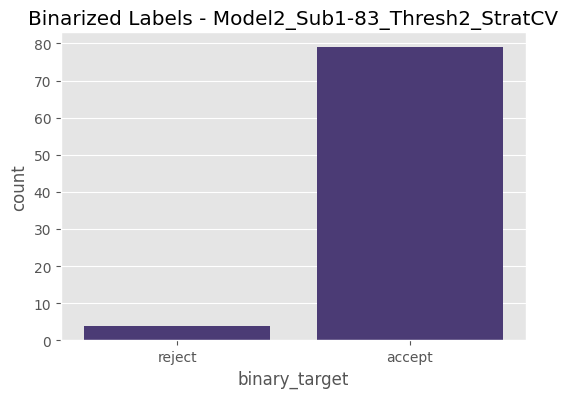
\includegraphics[width=0.40\textwidth]{Report/img/binary_scenario1_label_dist.png} 
        \caption{Distribution of binarized labels (Threshold 1).}
        \label{fig:binary_s1_labels}
\end{figure}

% \begin{figure}[H]
%     \centering
%     \begin{subfigure}[b]{0.48\textwidth}
%         \centering
%         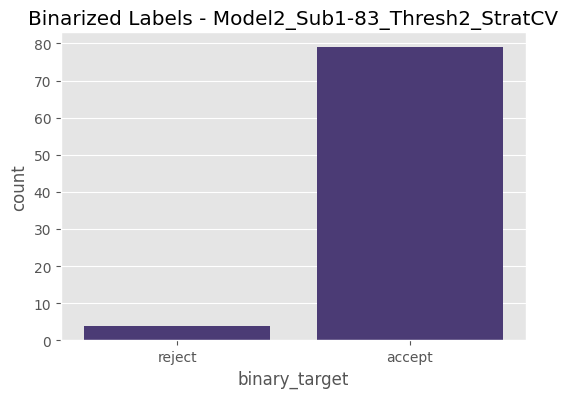
\includegraphics[width=\textwidth]{Report/img/binary_scenario1_label_dist.png} % Replace with your image path
%         \caption{Distribution of binarized labels (Threshold 1).}
%         \label{fig:binary_s1_labels}
%     \end{subfigure}
%     \hfill
%     \begin{subfigure}[b]{0.48\textwidth}
%         \centering
%         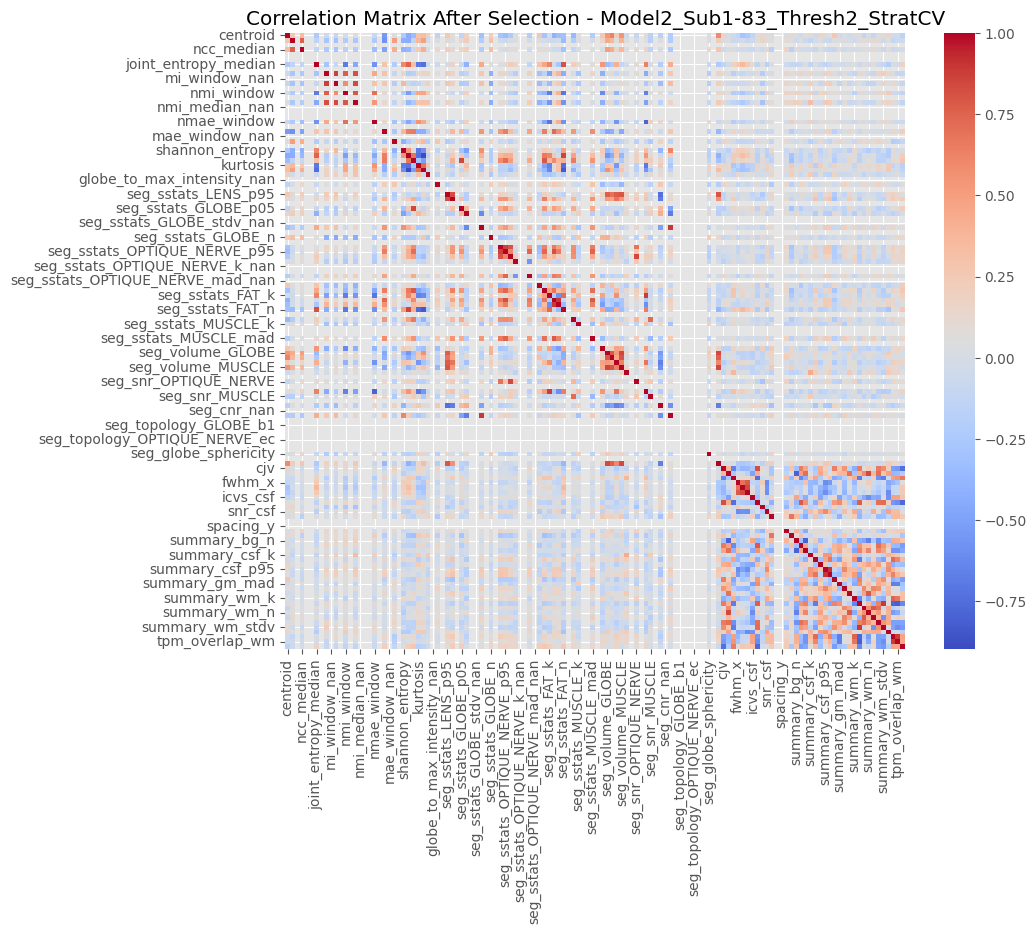
\includegraphics[width=\textwidth]{Report/img/binary_scenario_corr_matrix_selected.png} % Replace with your image path
%         \caption{Correlation matrix of selected IQMs.}
%         \label{fig:binary_s1_corr}
%     \end{subfigure}
%     \caption{Data characteristics for Binary Classification Scenario 1.}
%     \label{fig:binary_scenario1_distributions}
% \end{figure}

\subsubsection{Model Performance}
The performance of the \texttt{RandomForestClassifier} for this scenario is summarized in Table \ref{tab:binary_scenario1_metrics}. The confusion matrix and top 20 feature importances are shown in Figure \ref{fig:binary_scenario1_performance}. The model achieved an accuracy of 96\% and an F1-score of 0.98. The ROC AUC was 0.91. The most important features identified were FWHM\_z.
\begin{table}[H]
    \centering
    \caption{Evaluation Metrics for Binary Classification Scenario 1 (Threshold 1).}
    \label{tab:binary_scenario1_metrics}
    \begin{tabular}{lc}
        \toprule
        Metric & Value \\
        \midrule
        Accuracy (Agreement \%) & 21/1 96.0\% \\
        Balanced Accuracy & 50.0\% \\
        F1-Score & 0.98 \\
        Precision & 0.96 \\
        Recall & 1.00 \\
        ROC AUC & 0.91 \\
        \bottomrule
    \end{tabular}
\end{table}

\begin{figure}[H]
    \centering
    \begin{subfigure}[b]{0.4\textwidth}
        \centering
        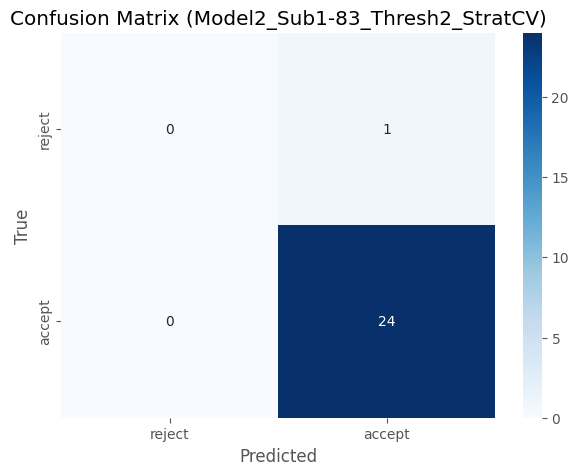
\includegraphics[width=\textwidth]{Report/img/binary_scenario1_confusion_matrix.png} % Replace with your image path
        \caption{Confusion matrix.}
        \label{fig:binary_s1_cm}
    \end{subfigure}
    \hfill
    \begin{subfigure}[b]{0.4\textwidth}
        \centering
        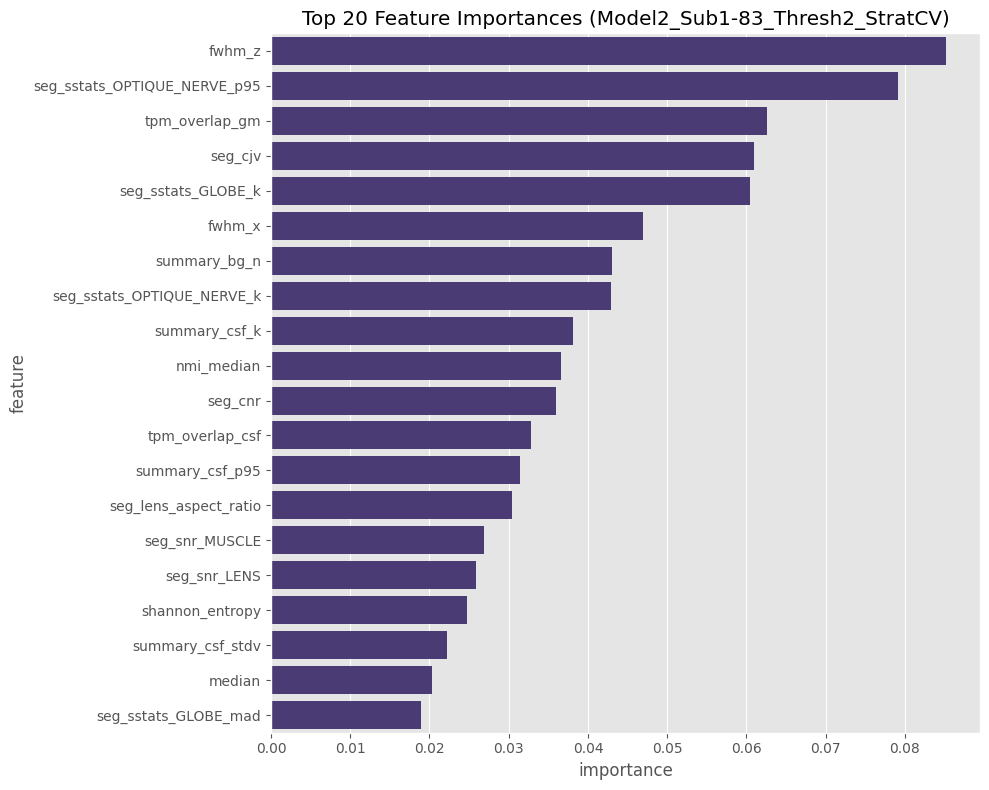
\includegraphics[width=\textwidth]{Report/img/binary_scenario1_feature_importance.png} % Replace with your image path
        \caption{Top 20 feature importances.}
        \label{fig:binary_s1_feat_imp}
    \end{subfigure}
    \caption{Performance visualizations for Binary Classification Scenario 1.}
    \label{fig:binary_scenario1_performance}
\end{figure}

\subsection{Scenario 2: Binary Classification - Threshold 2}
\label{ssec:binary_scenario2_results}

For this scenario, images were classified as "reject" if their continuous rating was less than 2 (i.e., "exclude" and "poor" classes), and "accept" otherwise (ratings $\geq 2$).

\subsubsection{Data Distribution}
As shown in figure \ref{fig:binary_s2_labels}, the distribution of classes is better proportioned.

\begin{figure}[h]
        \centering
        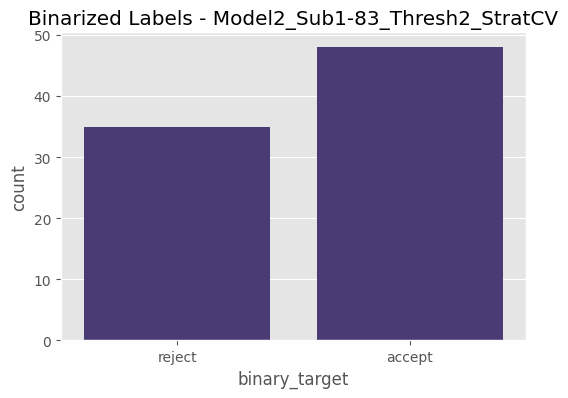
\includegraphics[width=0.4\textwidth]{Report/img/binary_scenario2_label_dist.png} 
        \caption{Distribution of binarized labels (Threshold 2).}
        \label{fig:binary_s2_labels}
\end{figure}

% \begin{figure}[H]
%     \centering
%     \begin{subfigure}[b]{0.48\textwidth}
%         \centering
%         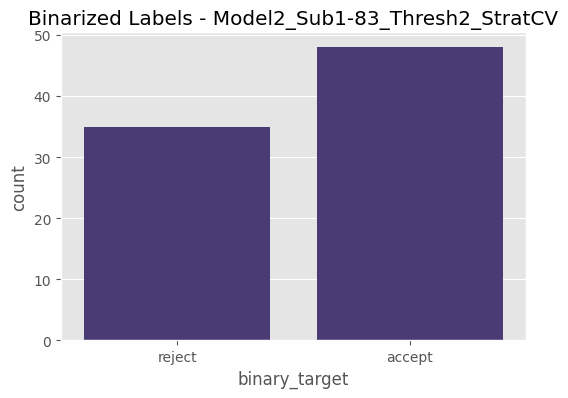
\includegraphics[width=\textwidth]{Report/img/binary_scenario2_label_dist.png} % Replace with your image path
%         \caption{Distribution of binarized labels (Threshold 2).}
%         \label{fig:binary_s2_labels}
%     \end{subfigure}
%     \hfill
%     \begin{subfigure}[b]{0.48\textwidth}
%         \centering
%         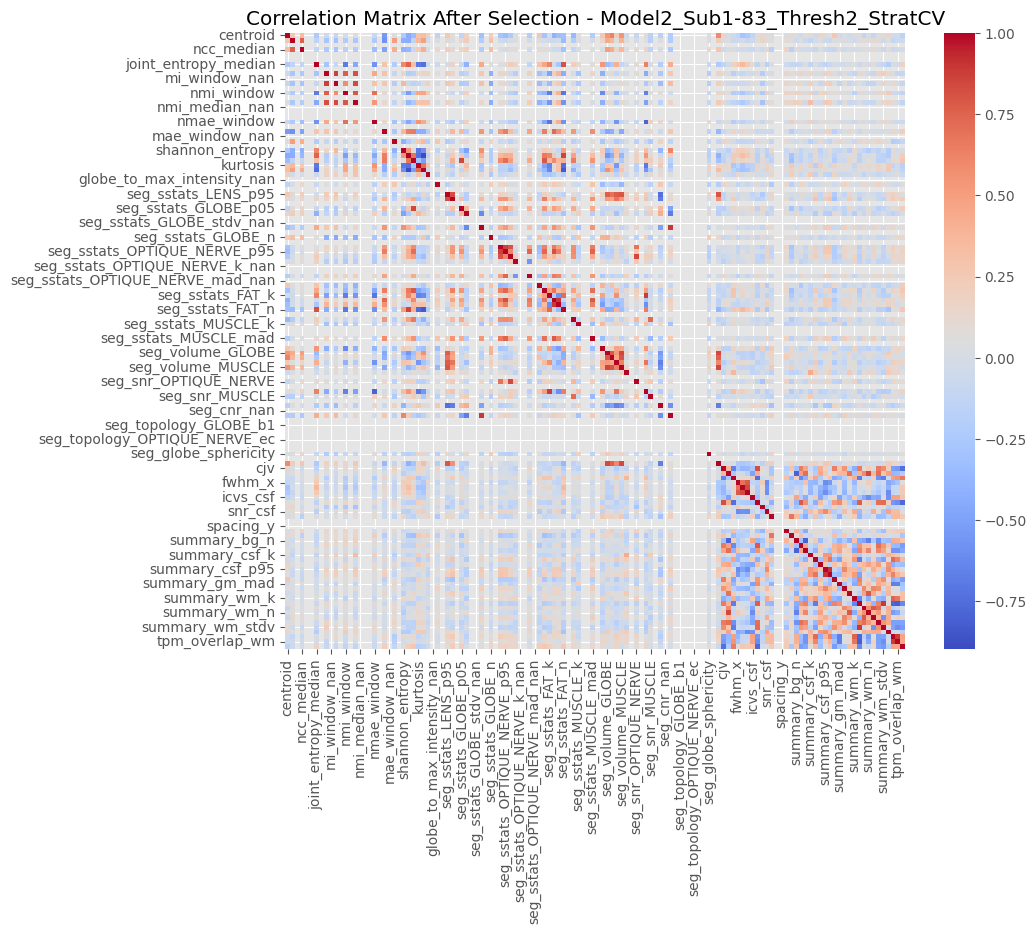
\includegraphics[width=\textwidth]{Report/img/binary_scenario2_corr_matrix_selected.png} % Replace with your image path
%         \caption{Correlation matrix of selected IQMs.}
%         \label{fig:binary_s2_corr}
%     \end{subfigure}
%     \caption{Data characteristics for Binary Classification Scenario 2.}
%     \label{fig:binary_scenario2_distributions}
% \end{figure}

\subsubsection{Model Performance}
The performance metrics are detailed in Table \ref{tab:binary_scenario2_metrics}, with the confusion matrix and feature importances in Figure \ref{fig:binary_scenario2_performance}. The model achieved an accuracy of 72\% and an F1-score of 0.75. The ROC AUC was 0.77. The most important features identified were SEG\_CJV.

\begin{table}[H]
    \centering
    \caption{Evaluation Metrics for Binary Classification Scenario 2 (Threshold 2).}
    \label{tab:binary_scenario2_metrics}
    \begin{tabular}{lc}
        \toprule
        Metric & Value \\
        \midrule
        Agreement \% & 18/7 72.0\% \\
        Balanced Accuracy & 71.1\% \\
        F1-Score & 0.75 \\
        Precision & 0.73 \\
        Recall & 0.78 \\
        ROC AUC & 0.77 \\
        \bottomrule
    \end{tabular}
\end{table}

\begin{figure}[H]
    \centering
    \begin{subfigure}[b]{0.45\textwidth}
        \centering
        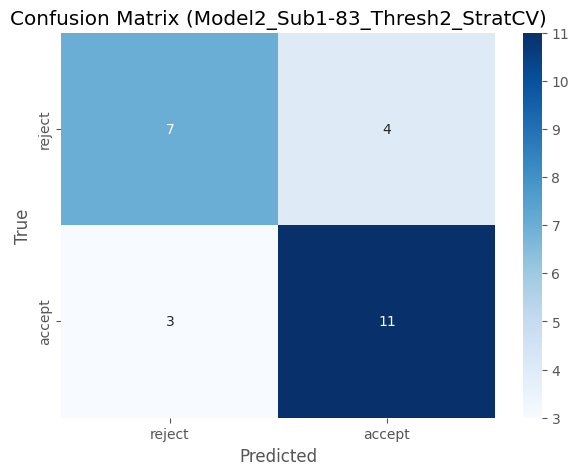
\includegraphics[width=\textwidth]{Report/img/binary_scenario2_confusion_matrix.png} % Replace with your image path
        \caption{Confusion matrix.}
        \label{fig:binary_s2_cm}
    \end{subfigure}
    \hfill
    \begin{subfigure}[b]{0.45\textwidth}
        \centering
        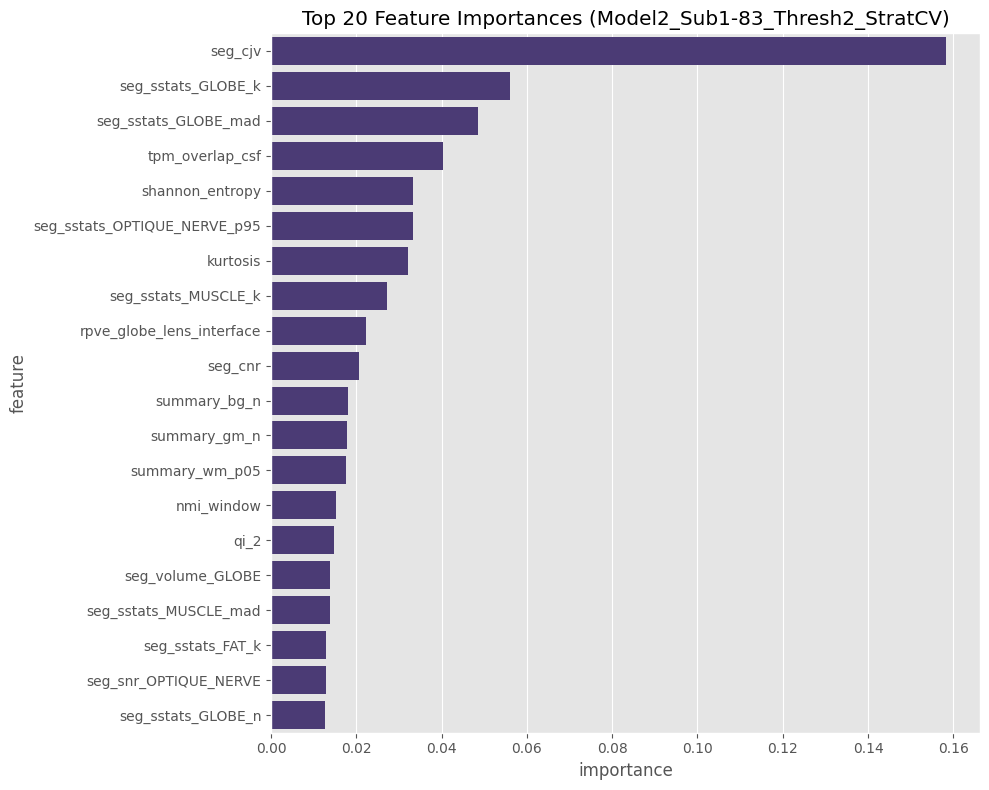
\includegraphics[width=\textwidth]{Report/img/binary_scenario2_feature_importance.png} % Replace with your image path
        \caption{Top 20 feature importances.}
        \label{fig:binary_s2_feat_imp}
    \end{subfigure}
    \caption{Performance visualizations for Binary Classification Scenario 2.}
    \label{fig:binary_scenario2_performance}
\end{figure}


\section{Multi-class Classification (with Binary Re-classification) Models}
\label{sec:multiclass_binary_results}
This approach involved first training a \texttt{RandomForestClassifier} to predict one of four quality classes ("exclude", "poor", "acceptable", "excellent"). The predicted multi-class labels were then mapped to a final binary "accept/reject" outcome.

\subsection{Scenario 3: Multi-class with Final Binary Grouping 1 (e.g., Reject = Exclude)}
\label{ssec:multiclass_scenario3_results}
In this scenario, for the final binary classification, only the "exclude" multi-class prediction was mapped to "reject", while "poor", "acceptable", and "excellent" were mapped to "accept".

\subsubsection{Data Distribution and Feature Correlation}
Figure \ref{fig:multiclass_scenario3_distributions} illustrates the distribution of the initial four multi-class labels, the distribution of the final binary labels after re-grouping, and the correlation matrix of selected IQMs.

\begin{figure}[H]
    \centering
    \begin{subfigure}[b]{0.45\textwidth}
        \centering
        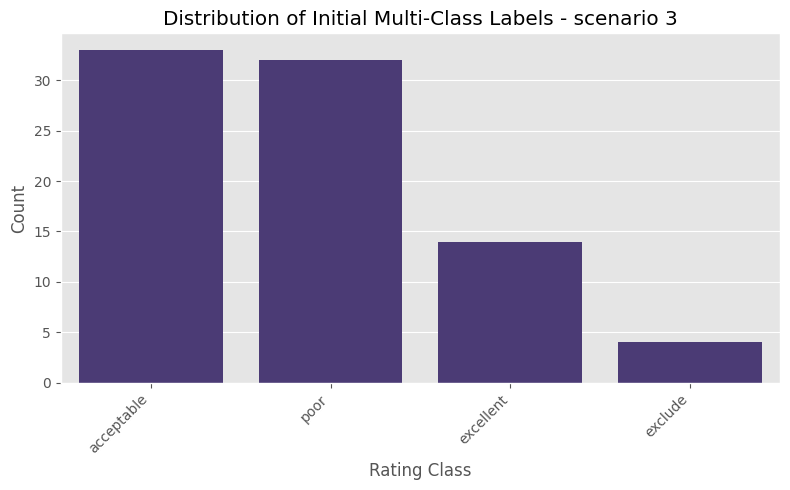
\includegraphics[width=\textwidth]{Report/img/multiclass_scenario3_label_dist.png} % Replace with your image path
        \caption{Multi-class labels.}
        \label{fig:multi_s3_multi_labels}
    \end{subfigure}
    \hfill
    \begin{subfigure}[b]{0.45\textwidth}
        \centering
        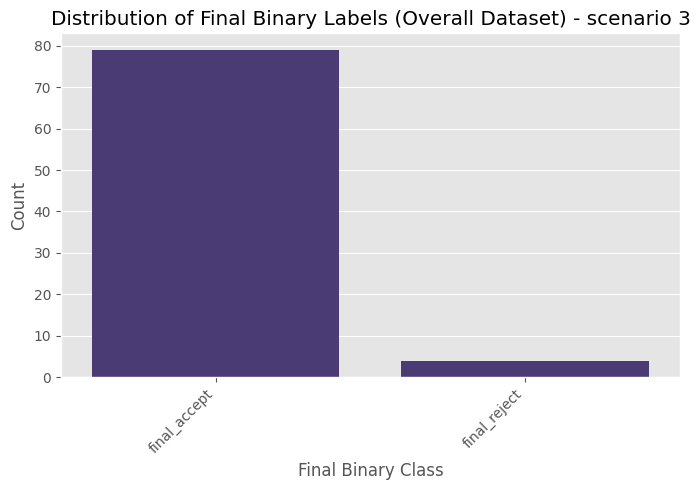
\includegraphics[width=\textwidth]{Report/img/multiclass_scenario3_label_dist_final.png} % Replace with your image path
        \caption{Final binary labels.}
        \label{fig:multi_s3_final_labels}
    \end{subfigure}
    \caption{Data characteristics for Multi-class Scenario 3.}
    \label{fig:multiclass_scenario3_distributions}
\end{figure}

\subsubsection{Model Performance}
The performance of the initial multi-class classification and the subsequent final binary classification are presented. Table \ref{tab:multiclass_scenario3_metrics} summarizes the key metrics. Figure \ref{fig:multiclass_scenario3_performance} shows the confusion matrices and feature importances. The model achieved an accuracy of 96\% and an F1-score of 0.75. The ROC AUC was 0.91. The most important features identified were SEG\_CJV.

\begin{table}[H]
    \centering
    \caption{Evaluation Metrics for Multi-class Scenario 3 (Reject = Exclude).}
    \label{tab:multiclass_scenario3_metrics}
    \begin{tabular}{lcc}
        \toprule
        Metric & Multi-class Stage & Final Binary Stage \\
        \midrule
        Accuracy (Agreement \%) & 17/8 68.0\% & 24/1 96.0\% \\
        Balanced Accuracy & 46.2\% & 50.0\% \\
        F1-Score (Macro/Binary) & 46.2 & 0.98 \\
        Precision (Macro/Binary) & 0.59 & 0.96 \\
        Recall (Macro/Binary) & 0.46 & 1.00 \\
        ROC AUC (OvR Macro/Binary) & 0.78 & 0.91 \\
        \bottomrule
    \end{tabular}
\end{table}

\begin{figure}[H]
    \centering
    \begin{subfigure}[b]{0.45\textwidth}
        \centering
        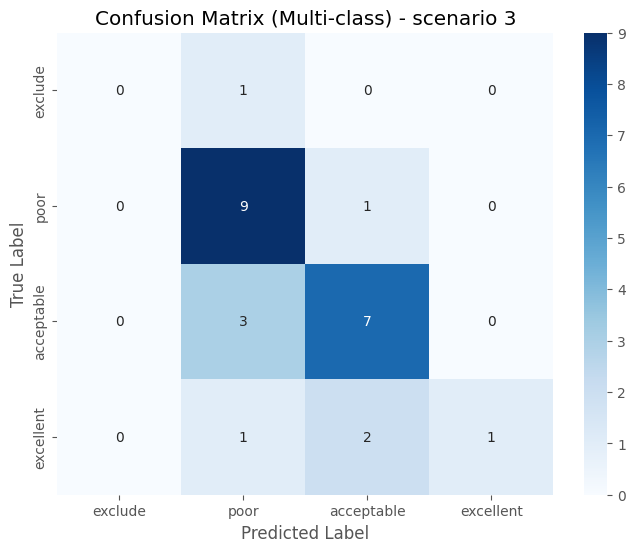
\includegraphics[width=\textwidth]{Report/img/multiclass_scenario3_corr_matrix_multi.png} % Replace with your image path
        \caption{Multi-class confusion matrix.}
        \label{fig:multi_s3_multi_cm}
    \end{subfigure}
    \hfill
    \begin{subfigure}[b]{0.45\textwidth}
        \centering
        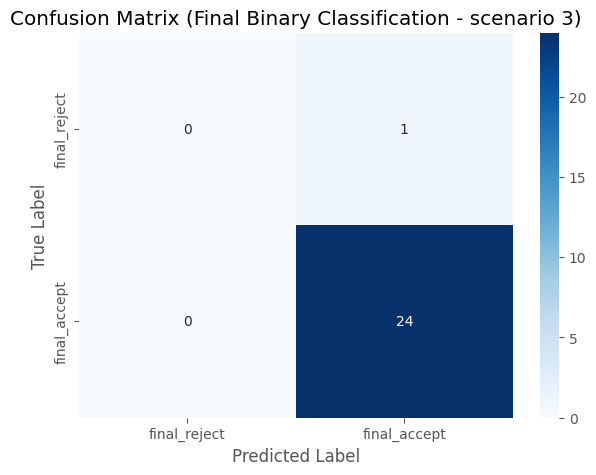
\includegraphics[width=\textwidth]{Report/img/multiclass_scenario3_corr_matrix.png} % Replace with your image path
        \caption{Final binary confusion matrix.}
        \label{fig:multi_s3_final_cm}
    \end{subfigure}
    \begin{subfigure}[b]{0.45\textwidth}
        \centering
        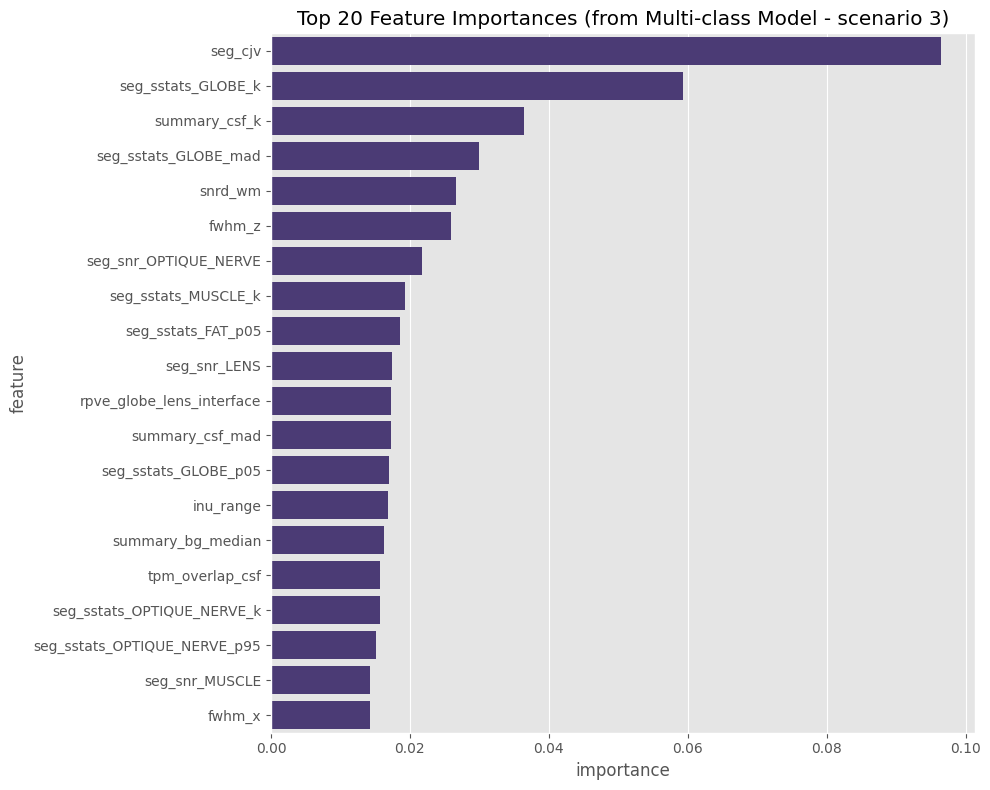
\includegraphics[width=\textwidth]{Report/img/multiclass_scenario3_feature_importance.png} % Replace with your image path
        \caption{Top 20 feature importances (from multi-class model).}
        \label{fig:multi_s3_feat_imp}
    \end{subfigure}
    \caption{Performance visualizations for Multi-class Scenario 3.}
    \label{fig:multiclass_scenario3_performance}
\end{figure}
\clearpage

\subsection{Scenario 4: Multi-class with Final Binary Grouping 2 (e.g., Reject = Exclude + Poor)}
\label{ssec:multiclass_scenario4_results}
In this scenario, for the final binary classification, both "exclude" and "poor" multi-class predictions were mapped to "reject", while "acceptable" and "excellent" were mapped to "accept".

\subsubsection{Data Distribution and Feature Correlation}
Figure \ref{fig:multiclass_scenario4_distributions} illustrates the label distributions and selected IQM correlations for this scenario.

\begin{figure}[H]
    \centering
    \begin{subfigure}[b]{0.45\textwidth}
        \centering
        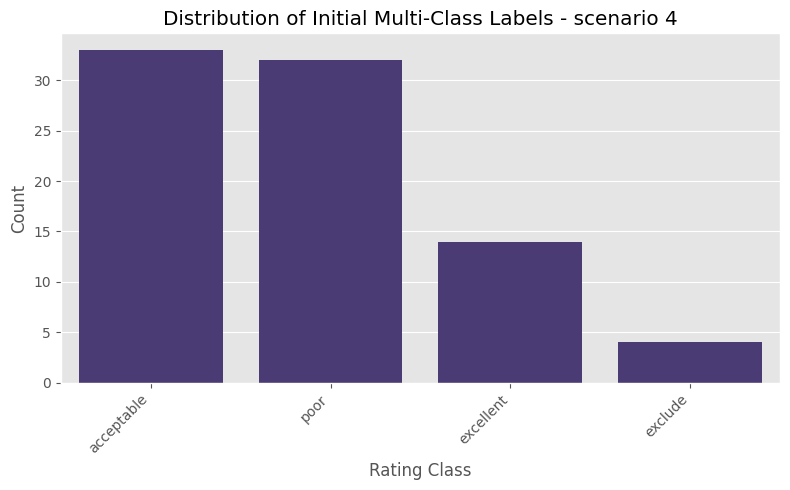
\includegraphics[width=\textwidth]{Report/img/multiclass_scenario4_lanel_dist.png} % Replace with your image path
        \caption{Multi-class labels.}
        \label{fig:multi_s4_multi_labels}
    \end{subfigure}
    \begin{subfigure}[b]{0.45\textwidth}
        \centering
        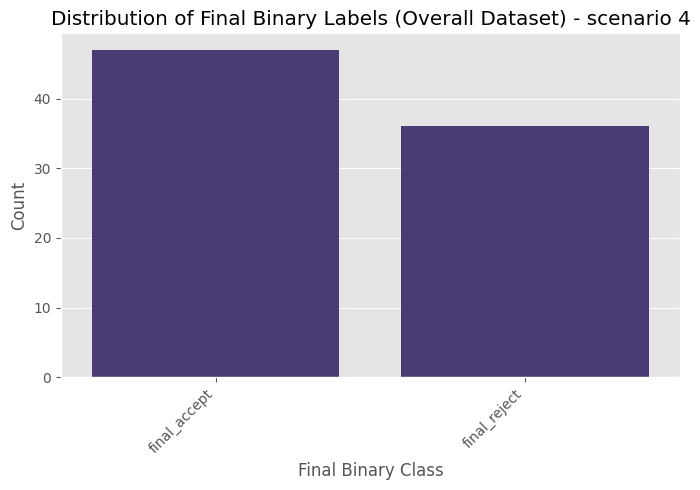
\includegraphics[width=\textwidth]{Report/img/multiclass_scenario4_label_dist_final.png} % Replace with your image path
        \caption{Final binary labels.}
        \label{fig:multi_s4_final_labels}
    \end{subfigure}
    \caption{Data characteristics for Multi-class Scenario 4.}
    \label{fig:multiclass_scenario4_distributions}
\end{figure}

\subsubsection{Model Performance}
Performance metrics are given in Table \ref{tab:multiclass_scenario4_metrics}, and visualizations in Figure \ref{fig:multiclass_scenario4_performance}.The model achieved an accuracy of 80\% and an F1-score of 0.80. The ROC AUC was 0.91. The most important features identified were SEG\_CJV.

\begin{table}[H]
    \centering
    \caption{Evaluation Metrics for Multi-class Scenario 4 (Reject = Exclude + Poor).}
    \label{tab:multiclass_scenario4_metrics}
    \begin{tabular}{lcc}
        \toprule
        Metric & Multi-class Stage & Final Binary Stage \\
        \midrule
        Accuracy (Agreement \%) & 17/8 68.0\% & 25/5 80.0\% \\
        Balanced Accuracy & 46.25\% & 81.1\% \\
        F1-Score (Macro/Binary) & 0.46 & 0.80 \\
        Precision (Macro/Binary) & 0.90 & 0.90 \\
        Recall (Macro/Binary) & 0.59 & 0.71 \\
        ROC AUC (OvR Macro/Binary) & 0.79 & 0.91 \\
        \bottomrule
    \end{tabular}
\end{table}

\begin{figure}[H]
    \centering
    \begin{subfigure}[b]{0.445\textwidth}
        \centering
        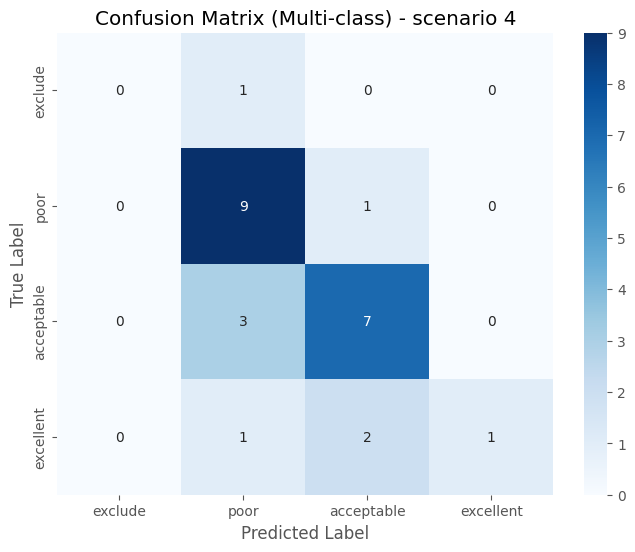
\includegraphics[width=\textwidth]{Report/img/multiclass_scenario4_confusion_matrix_multi.png} % Replace with your image path
        \caption{Multi-class confusion matrix.}
        \label{fig:multi_s4_multi_cm}
    \end{subfigure}
    \hfill
    \begin{subfigure}[b]{0.45\textwidth}
        \centering
        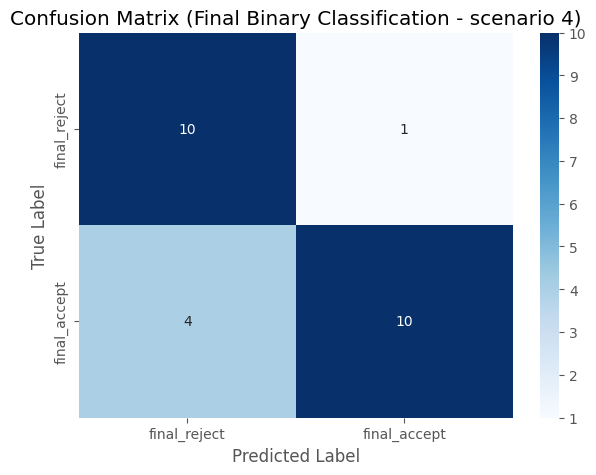
\includegraphics[width=\textwidth]{Report/img/multiclass_scenario4_confusion_matrix.png}
        \caption{Final binary confusion matrix.}
        \label{fig:multi_s4_final_cm}
    \end{subfigure}
    \begin{subfigure}[b]{0.45\textwidth}
        \centering
        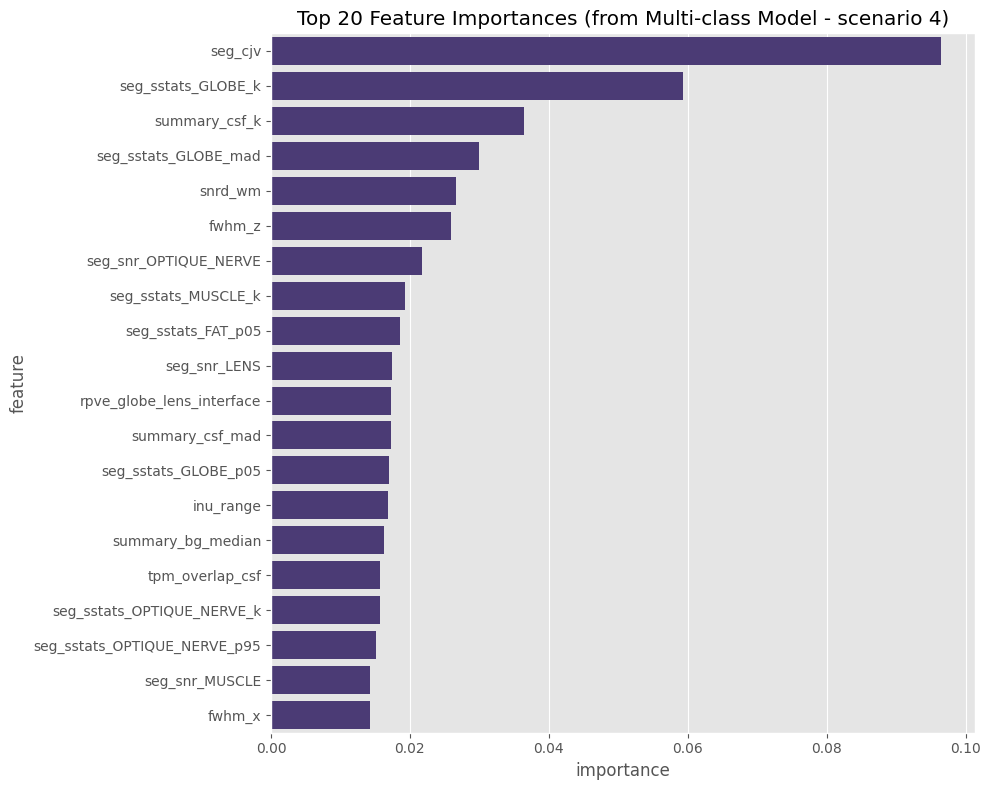
\includegraphics[width=\textwidth]{Report/img/multiclass_scenario4_feature_importance.png} % Replace with your image path
        \caption{Top 20 feature importances (from multi-class model).}
        \label{fig:multi_s4_feat_imp}
    \end{subfigure}
    \caption{Performance visualizations for Multi-class Scenario 4.}
    \label{fig:multiclass_scenario4_performance}
\end{figure}
\clearpage

\section{Comparative Analysis and Discussion}
\label{sec:comparative_analysis_results}

This section provides a comparative overview of the performance across all four scenarios, focusing on the final binary "accept/reject" classification task.

\begin{table}[H]
    \centering
    \caption{Comparison of Final Binary Classification Metrics Across All Scenarios.}
    \label{tab:all_scenarios_comparison}
    \begin{tabular}{lcccc}
        \toprule
        Metric & Binary Scen. 1 & Binary Scen. 2 & Multi-class Scen. 3 & Multi-class Scen. 4 \\
        & (Thresh 1) & (Thresh 2) & (Reject=Excl) & (Reject=Excl+Poor) \\
        \midrule
        Accuracy & 21/1 96.0\% & 18/7 72.0\% & 24/1 96.0\% & 25/5 80.0\% \\
        Balanced Acc. & 50.0\% & 71.1\% & 50.0\% & 81.1\% \\
        F1-Score & 0.98 & 0.75 & 0.98 & 0.80 \\
        Precision & 0.96 & 0.73 & 0.96 & 0.90 \\
        Recall & 1.00 & 0.78 & 1.00 & 0.71 \\
        ROC AUC & 0.91 & 0.77 & 0.91 & 0.91 \\
        % Add other relevant metrics
        \bottomrule
    \end{tabular}
\end{table}

\textbf{The Effect of Severe Class Imbalance on Model Performance}

A primary observation pertains to Scenarios 1 and 3, which were characterized by a severe class imbalance. In Scenario 1 (direct binary classification), the dataset contained 21 "accept" cases versus only one "reject" case. Similarly, Scenario 3 (regression-based model) had a 24-to-1 ratio. For both scenarios, the models achieved a high standard Accuracy (96.0\%) but a Balanced Accuracy of exactly 50.0\%.

A balanced accuracy of 50\% in a binary classification task indicates that the model's performance is equivalent to random chance. The discrepancy with the high standard accuracy is a classic symptom of a model trained on imbalanced data. The model learns that the most effective strategy to minimize overall error is to almost always predict the majority class ("accept"). Consequently, it correctly classifies the vast majority of cases but completely fails to identify the minority "reject" class. This is further evidenced by the Recall of 1.00 for the majority class in these scenarios. Due to their inability to generalize and identify the crucial "reject" cases, these models are considered unusable for practical quality control.

Interestingly, the ROC AUC for these scenarios remained high (0.91). This suggests that while the default classification threshold (0.5) leads to poor performance, the models have learned a probabilistic separation between the classes. With appropriate threshold tuning, it might be possible to improve performance, but the fundamental issue remains the lack of sufficient data for the minority class.

\textbf{Comparison of Modeling Strategies and Classification Scenarios}

The four scenarios were designed to compare two distinct modeling approaches: direct binary classification (Scenarios 1 and 2), where the model is trained to predict a binary label (0 or 1), and a regression-based approach (Scenarios 3 and 4), where the model is first trained to predict a continuous quality value, which is then binarized using a threshold.

When comparing the more balanced datasets (Scenarios 2 and 4), a significant performance difference emerges between these two strategies.
\begin{itemize}
    \item \textbf{Scenario 2 (Direct Binary Classification):} With a more balanced dataset (18 "accept" vs. 7 "reject"), this model achieved a substantial Balanced Accuracy of 71.1\%, demonstrating its ability to learn distinguishing features beyond simply predicting the majority class.
    \item \textbf{Scenario 4 (Regression-to-Classification):} This approach, which also used a balanced dataset (25 "accept" vs. 5 "reject"), yielded the best overall results, achieving a superior Balanced Accuracy of 81.1\%.

\end{itemize}
This comparison strongly suggests that training the model to predict a continuous quality score first provides a richer learning signal. This regression task likely leverages the nuance of the multi-class ratings (e.g., the difference between "poor", "acceptable", and "excellent"). The subsequent binarization of this more informed, continuous output into a simple "accept/reject" decision is more effective than training the model on a pre-binarized target from the outset. This demonstrates that for this dataset, a regression-to-classification approach is the superior strategy.

\textbf{Analysis of Informative Image Quality Metrics (IQMs)}

An analysis of the feature importances from the Random Forest models in the successful Scenarios (2 and 4) reveals a consistent pattern: the most predictive IQMs are those derived from anatomical segmentations, rather than global image statistics.

This is a critical finding, as it implies that the quality of the image is best reflected in the characteristics of the segmented ocular structures themselves. The high ranking of metrics related to the GLOBE and LENS suggests that the morphology, intensity contrast, and signal homogeneity of these specific tissues are powerful indicators of overall image quality. This underscores the importance of accurate, high-quality segmentation as a prerequisite for effective automated QC.

Of particular note is the consistent high importance of seg\_CJV (Coefficient of Joint Variation). In all evaluated models, this metric ranked within the top two most influential features. The CJV quantifies the relationship between signal variability (noise) and the contrast between the lens and the globe. Its high predictive power suggests that this ratio is exceptionally sensitive to image degradations, potentially capturing subtle effects of motion, noise, or intensity non-uniformities that other metrics miss. While its dominance is striking, it warrants further investigation to confirm that its high values are not an artifact of a specific data characteristic and to fully understand the quality-related phenomena it so effectively captures.

% Figure \ref{fig:scenario_comparison_plots} visually compares key performance metrics (e.g., F1-score and ROC AUC for the final binary classification) across the four scenarios.

% \begin{figure}[H]
%     \centering
%     \begin{subfigure}[b]{0.48\textwidth}
%         \centering
%         \includegraphics[width=\textwidth]{path/to/all_scenarios_f1_comparison.png} % Replace with your image path
%         \caption{Comparison of F1-Scores (Final Binary).}
%         \label{fig:all_s_f1}
%     \end{subfigure}
%     \hfill
%     \begin{subfigure}[b]{0.48\textwidth}
%         \centering
%         \includegraphics[width=\textwidth]{path/to/all_scenarios_roc_auc_comparison.png} % Replace with your image path
%         \caption{Comparison of ROC AUC (Final Binary).}
%         \label{fig:all_s_roc}
%     \end{subfigure}
%     \caption{Comparative performance plots across all scenarios for the final binary classification.}
%     \label{fig:scenario_comparison_plots}
%\end{figure}

